\documentclass{article}
\usepackage{amsmath}
\usepackage{graphicx}
\usepackage{verbatim}
\usepackage{color}   %May be necessary if you want to color links
\usepackage{hyperref}
\usepackage[utf8]{inputenc}
\usepackage{tikz}
\usetikzlibrary{shapes.geometric,arrows}

\tikzstyle{startstop}=[rectangle,rounded corners,minimum width=3cm,
minimum height=1cm,text centered,draw=black,fill=red!30]
\tikzstyle{io}=[trapezium,trapezium left angle=70, trapezium right angle= 110,minimum width=6cm,
minimum height=1cm,text centered,draw=black,fill=blue!30]
\tikzstyle{process}=[rectangle,minimum width=3cm,
minimum height=1cm,text centered,text width=3cm,draw=black,fill=orange!30]
\tikzstyle{decision}=[diamond,minimum width=3cm,
minimum height=1cm,text centered,draw=black,fill=green!30]
\tikzstyle{arrow}=[thick,->,>=stealth]

\hypersetup{
    colorlinks=true, %set true if you want colored links
    linktoc=all,     %set to all if you want both sections and subsections linked
    linkcolor=blue,  %choose some color if you want links to stand out
}
\begin{document}
    \begin{titlepage}
        \begin{center}
            \vspace*{0cm}
            \Huge
            \textbf{ELP780}
     
            \vspace{0.5cm}
            \LARGE
            Software Lab
     
            \vspace{1.5cm}
            \textbf{Aghil Sabu\\}

            \vspace{.3cm}
            2018EET2865
     
            \vfill
            A report presented for the assignment on\\
            Assignment 8 - Python and Github 
     
            \vspace{0.8cm}
            
\includegraphics[width=0.45\textwidth]{./images/logo}
     
            \Large
            Electrical Engineering\\
            IIT Delhi\\
            India\\
            \today
        \end{center}
    \end{titlepage}
    \tableofcontents
    \pagenumbering{arabic}
    \pagebreak
    
    \section{Problem Satement 1}
    \subsection{Problem Statement}
    You have a file with the contents of players’ names and their scores. Create a programme using
Lex(flex) to calculate total runs scored by the players. Also calculate their averages.
Sample File Format is as below
\\Input Format:
$$./ps1 <input_file>$$
Output Format:
$$<player_name> <Total_run> <average>$$
% \end{itemize}
    \subsection{PS1 algorithm}
    \begin{itemize}
        \item Read filename from user
        \item read words and numbers separately
        \item for each ney name if name does't already exist, add name
        \item add score for respective name
        \item calculate sum and average
        \item display rsults in the required format
    \end{itemize}
    \subsection{PS1 Flow Chart}
    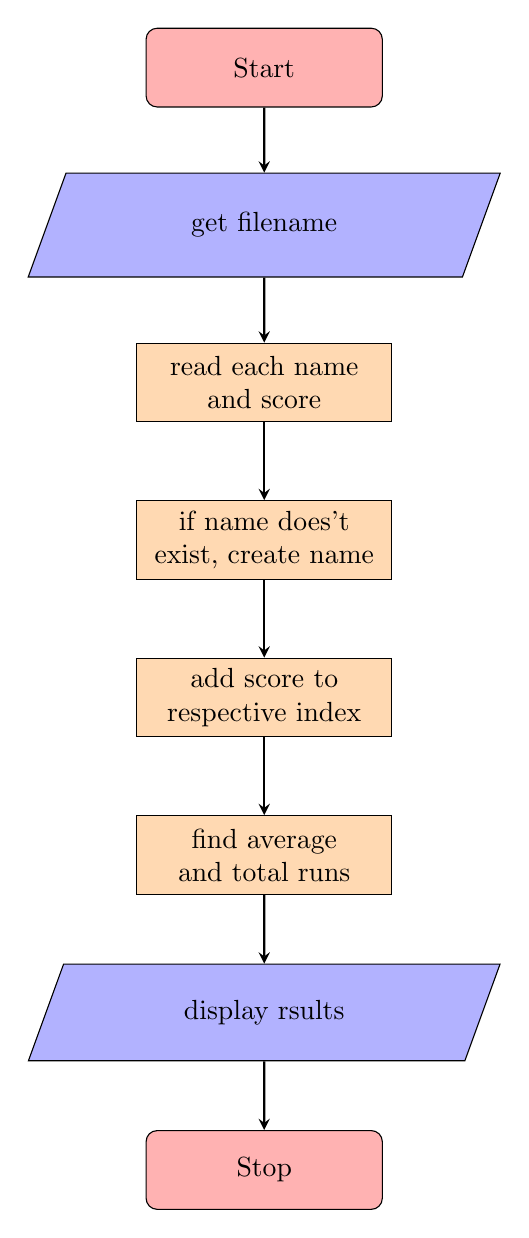
\begin{tikzpicture}[node distance=2cm]
        \node (start) [startstop] {Start};
        \node (p1) [io,below of=start] {get filename};
        \node (p2) [process,below of=p1] {read each name and score};
        \node (p3) [process,below of=p2] {if name does't exist, create name};
        \node (p4) [process,below of=p3] {add score to respective index};
        \node (p5) [process,below of=p4] {find average and total runs};
        \node (p6) [io,below of=p5] {display rsults};
        \node (stop) [startstop,below of=p6] {Stop};

    
        \draw [arrow] (start) -- (p1);
        \draw [arrow] (p1) -- (p2);
        \draw [arrow] (p2) -- (p3);
        \draw [arrow] (p3) -- (p4);
        \draw [arrow] (p4) -- (p5);
        \draw [arrow] (p5) -- (p6);
        \draw [arrow] (p6) -- (stop);
    
    
    
    \end{tikzpicture}
    \pagebreak
    \subsection{PS1 Solution-Code}
    \verbatiminput{ps1.l}
    
    \pagebreak
    \subsection{PS1 Output Screenshots}
    \begin{center}     
        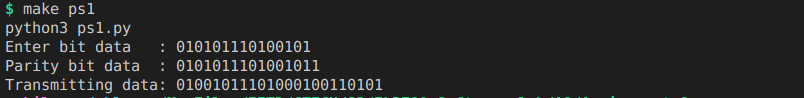
\includegraphics[width=1.1\textwidth]{./images/ps1_001.png}
    \end{center}
    \pagebreak
    \section{Problem Satement 2}
    A 8085 assembler is designed in a way that it takes input assembly source code instructions in
all capital letters and numbers in hexadecimal format suffixed by H.
You have to create preprocessor for assembler that will translate any 8085 assembly code into
full capital letters and all numerals into hexadecimal format suffixed by H.
Use lex(flex) and Yacc(bison).
        
    \subsection{PS2 algorithm}
    \begin{itemize}
        \item Get filenames from user
        \item for each line get all characters before colon ':'
        \item make all uppercase
        \item add hexadecimal 'H' wherever required
        \item save result to output file
    \end{itemize}
    \subsection{PS2 Flow Chart}
    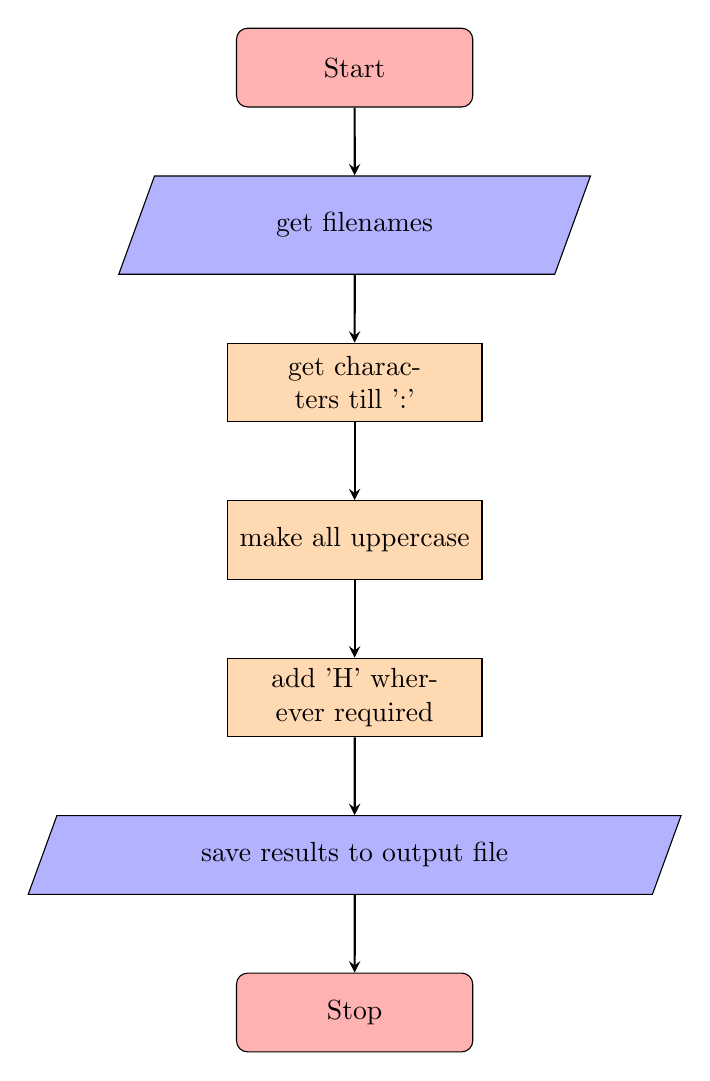
\begin{tikzpicture}[node distance=2cm]
        \node (start) [startstop] {Start};
        \node (p1) [io,below of=start] {get filenames};
        \node (p2) [process,below of=p1] {get characters till ':'};
        \node (p3) [process,below of=p2] {make all uppercase};
        \node (p4) [process,below of=p3] {add 'H' wherever required};
        \node (p5) [io,below of=p4] {save results to output file};
        \node (stop) [startstop,below of=p5] {Stop};

    
        \draw [arrow] (start) -- (p1);
        \draw [arrow] (p1) -- (p2);
        \draw [arrow] (p2) -- (p3);
        \draw [arrow] (p3) -- (p4);
        \draw [arrow] (p4) -- (p5);
        \draw [arrow] (p5) -- (stop);
    
    
    
    \end{tikzpicture}
    \pagebreak
    \subsection{PS2 Solution-Code}
    \verbatiminput{ps2.l}

    \pagebreak
    \subsection{PS2 Output }
    \subsubsection{input file}
    \verbatiminput{ps2.txt}
    \subsubsection{output file}
    \verbatiminput{output.txt}
    % 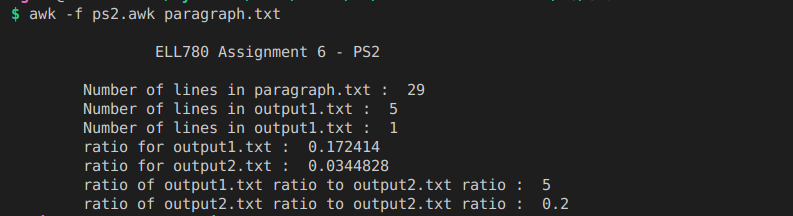
\includegraphics[width=1.2\textwidth]{./images/ps2_001.png}
    \pagebreak
    \section{makefile}
    \subsection{makefile code}
    \verbatiminput{makefile}
    % \subsection{makefile Screenshots}
    % 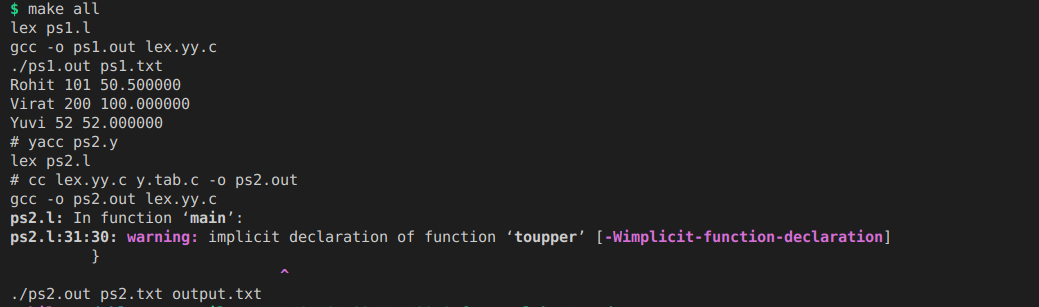
\includegraphics[width=1.2\textwidth]{./images/mk_001.png}
    \subsection{makefile output}
    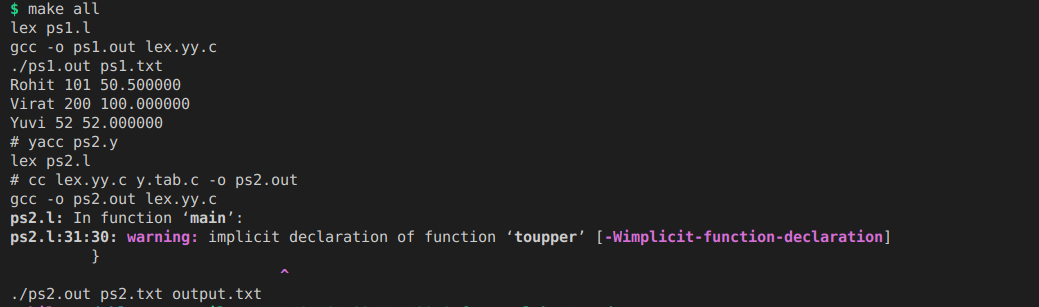
\includegraphics[width=1.2\textwidth]{./images/mk_001.png}


    \section{GIT}
    \subsection{GIT Commit Screenshots}
    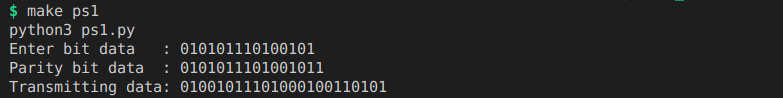
\includegraphics[width=1.2\textwidth]{./images/gt_001.png}
    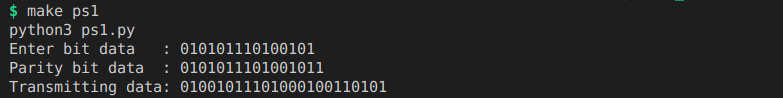
\includegraphics[width=1.2\textwidth]{./images/gt_001.png}

\end{document}